\usepackage{subcaption}
\documentclass{article}
\usepackage{booktabs}
\usepackage{graphicx}
\usepackage{amsmath}
\usepackage[a4paper, total={6.5in, 9.5in}]{geometry}
\usepackage{hyperref}
\usepackage{float}

\title{Previous Relationships vs Match Rate}
\author{Group 6}
\date{April 2025}

\begin{document}

\maketitle

\begin{table}[ht]
    \centering
    \begin{tabular}{ccc} 
    \toprule
    \textbf{First Name} & \textbf{Last Name} & \textbf{Student Number} \\ 
    \midrule
    Dean & Kuurstra    & s3343715 \\ 
    Diego & Cañas Jimenez & s3856216 \\
    Koorosh & Komeili Zadeh & s3893995 \\ 
    Lani & Hampel & s3977412 \\ 
    \bottomrule
    \end{tabular}
    \label{tab:group6_members}
\end{table}

\section{Introduction}

According to Stanford University Libraries (2023) \cite{rosenfeld2023}, the most common way couples meet is through online dating. This makes online dating a relevant topic of study and interest. To further understand online dating, it is worth considering distinct variables and their effect on the number of matches a user receives. This paper will investigate how the number of previous user relationships influences their match rates. This may provide further insight into the most common method currently used to find relationships. Furthermore, research into this topic may uncover unknown trends with less obvious features, one of which could be the aforementioned number of previous relationships and a user’s likelihood of successfully finding a match through online dating. Additionally, this paper aims examine the impact of using questionable research practices by using our data (QRP). Specifically, the impact of rounding p-values, discarding outliers and using sequential testing with optional stopping will be investigated.


\section{Previous Relationships vs Match Rate}

\subsection{Exploration}

% Simplify and shorten the paragraph

It is interesting to explore the relationship between the number of previous relationships and match rate, as reasonable arguments can defend both (positive and negative) trends. Our study aims to uncover this relationship. For this, we use the number of previous relationships as an explanatory variable, and we use the match rate as the response variable. We aim to examine the relationship through linear regression and thus answer whether the previous number of relationships affects the match rate of the users, whether this effect is positive or negative, if it is indeed present, and how strong this relationship is. 

\subsection{Methodology}

Our study aims to uncover the relationship between the number of previous relationships and match rate. For this relationship, we use the number of previous relationships as an explanatory variable, and we use the match rate as the response variable. We aim to examine the relationship through linear regression and thus answer whether the previous number of relationships affects the match rate of the users, whether this effect is positive or negative, if it is indeed present, and how strong this relationship is. 

\subsection{Hypothesis}

The Null Hypothesis suggests there is no direct connection between the number of previous significant relationships and the said user's match rate. Thereby, the linear regression’s slope ($\beta$) is zero. The alternative hypothesis suggests that there exists a correlation between the two variables. In other words, $\beta$ is non-zero. Thereby, this is a two-sided test.

\[
H_0: \beta = 0
\]

\[
H_a: \beta \neq 0
\]

The alpha value will be set to 0.05.

\subsection{Data Gathering}
For this project, data for both of our quantitative variables were randomly generated using a normal distribution, partially based on information found online. The standard mean and standard deviation for the normal curve that gives the match are 0.10\cite{elad2024} and 0.15, respectively. The distribution gives the number of previous serious relationships is which breaks the mean of 3 and the standard deviation of 4. The random values that exceeded the limits, namely 0 and 1 for match rate and 0 and 12, were truncated to the closest limit. Ten thousand tests were developed, each containing 5280 data points. 

\subsection{Findings and Analysis}

A linear regression was drawn for every test, and a slope and p-value were obtained by using the linear regression model. The linear regression model uses a t-test and the standard error. The p-values were then plotted in a histogram with a separation of 0.05.


\begin{figure}
    \centering
    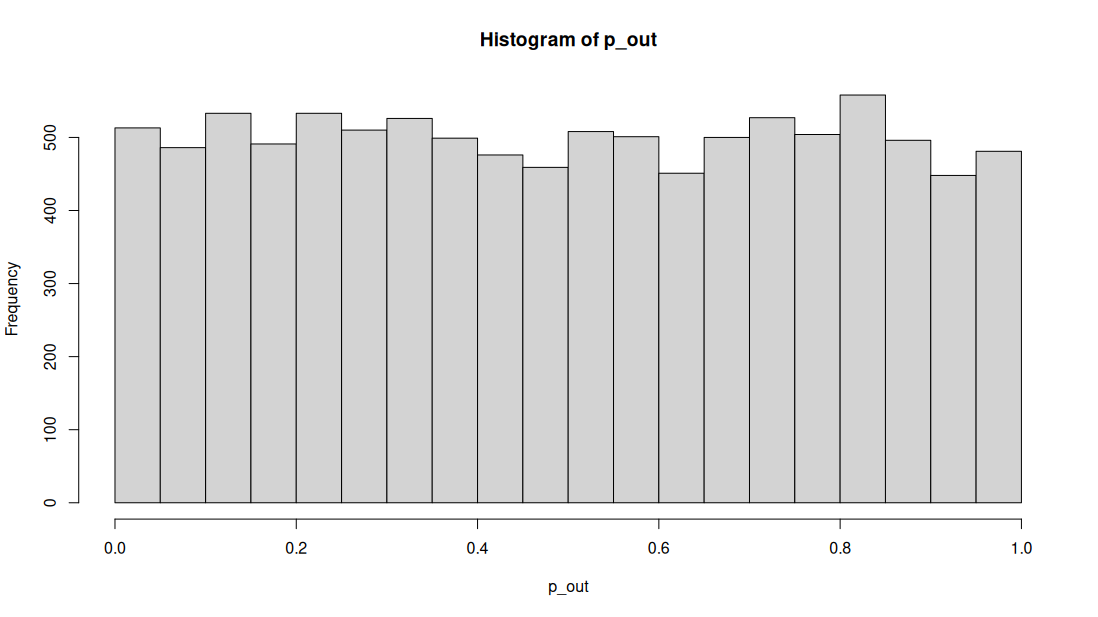
\includegraphics[width=1\linewidth]{Assignment1/figures/plot.png}
    \caption{The histogram shows the distribution of the p-values with their respective densities(related to the frequencies or number of occurrences) in 10.000 tests and a separation of 0.05.}
    \label{fig:enter-label}
\end{figure}

Each bin in the histogram represents a range of 0.05 p-values. All bins have a similar probability, namely about 5\%. This value can be obtained by finding the area of the bins. The expected value of false positives for two-sided tests is equivalent the alpha value, namely 0.1, as there are at least two extremes that are as extreme as alpha. The first and last bins represent the false positives as they are at least as extreme as the alpha value (0.05). These extremes give a total area close to 0.1, which approximately matches the expected value.

\section{Impact of using QRP}

\section{Impact of Rounding P-values}

This section visualizes the effect of rounding p-values, a questionable research practice (QRP), on statistical results. Rounding p-values above 0.05 to 0.05 can increase the number of significant results, making false positives increase and inaccurate scientific conclusions. The exploration shows that different p-value ranges (0.05–0.06, 0.05–0.07, 0.05–0.08, and 0.05–0.09) affect the distribution of p-values.

\begin{figure}[h!]
    \centering
    \begin{minipage}{0.45\textwidth}
        \centering
        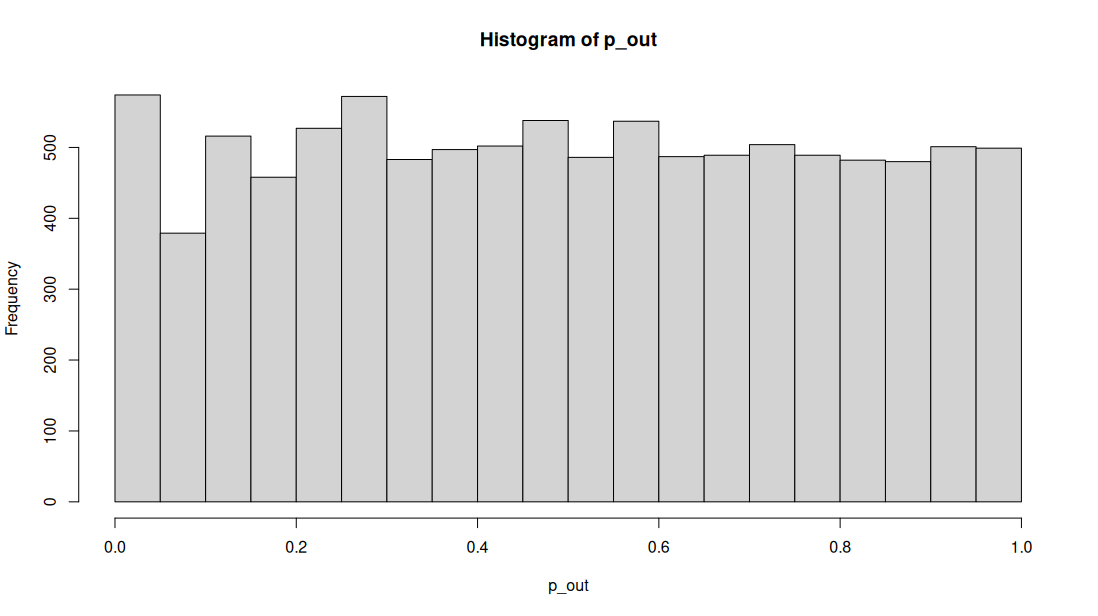
\includegraphics[width=\textwidth]{Assignment1/p-round/06.png}
        \caption{Range 0.05 to 0.06 rounded to 0.05}
    \end{minipage} \hfill
    \begin{minipage}{0.45\textwidth}
        \centering
        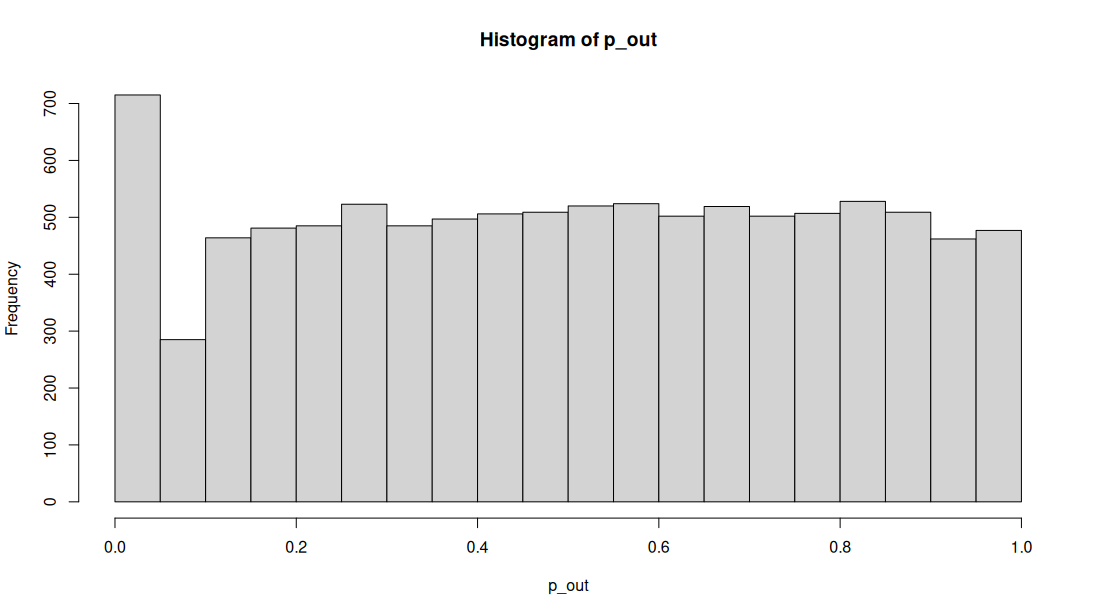
\includegraphics[width=\textwidth]{Assignment1/p-round/07.png}
        \caption{Range 0.05 to 0.07 rounded to 0.05}
    \end{minipage}

    \vskip\baselineskip

    \begin{minipage}{0.45\textwidth}
        \centering
        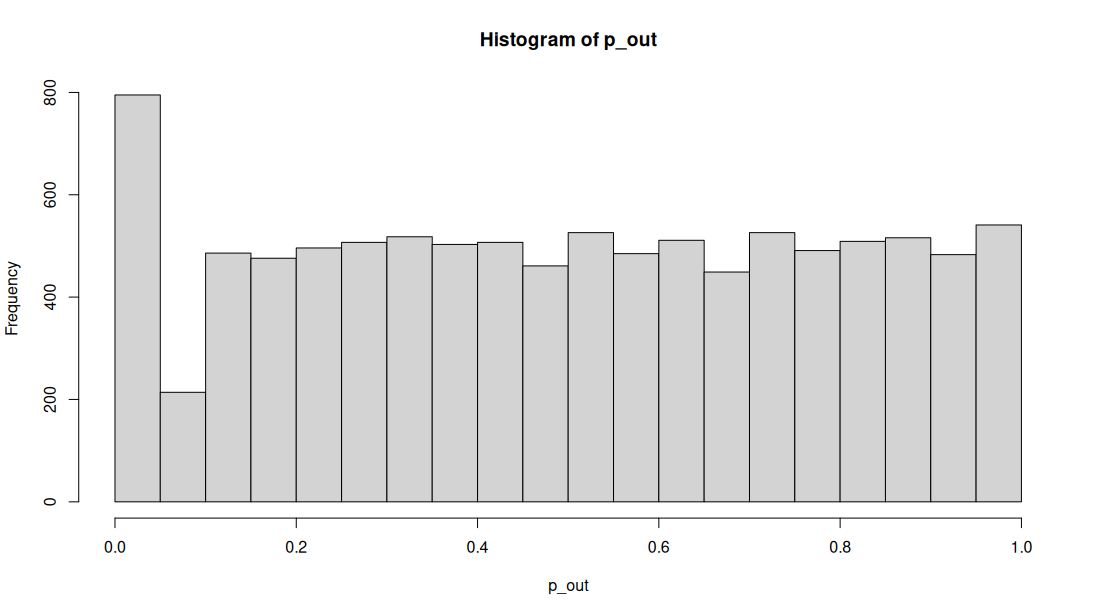
\includegraphics[width=\textwidth]{Assignment1/p-round/08.png}
        \caption{Range 0.05 to 0.08 rounded to 0.05}
    \end{minipage} \hfill
    \begin{minipage}{0.45\textwidth}
        \centering
        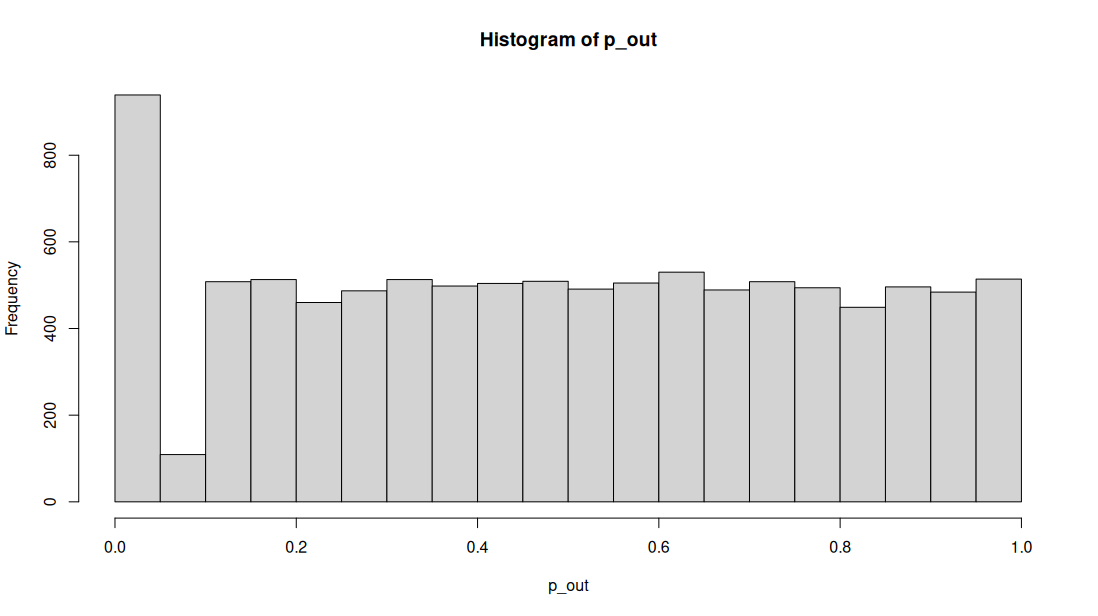
\includegraphics[width=\textwidth]{Assignment1/p-round/09.png}
        \caption{Range 0.05 to 0.09 rounded to 0.05}
    \end{minipage}
\end{figure}

Rounding p-values increases the Type I error rate by making non-significant results, which can cause incorrect replication and have an impact on the reliability and integrity of scientific research.



\bibliographystyle{IEEEtran}
\bibliography{references}

\end{document}
